%----------------------------------------------------------------------------------------
%	PACKAGES AND OTHER DOCUMENT CONFIGURATIONS
%----------------------------------------------------------------------------------------
\documentclass[fleqn,9 pt]{SelfArx} % Document font size and equations flushed left

% Decrease margins
%\addtolength{\oddsidemargin}{-0.3 in}
%\addtolength{\evensidemargin}{0 in}
%\addtolength{\textwidth}{0.8 in}
%\addtolength{\topmargin}{-0.5 in}
%\addtolength{\textheight}{1 in}

\usepackage[english]{babel} % Specify a different language here - english by default
\usepackage{lipsum} % Required to insert dummy text. To be removed otherwise
\usepackage{listings}
\usepackage{lipsum}  
\usepackage{caption}

%----------------------------------------------------------------------------------------
%	COLUMNS
%----------------------------------------------------------------------------------------
\setlength{\columnsep}{0.55cm} % Distance between the two columns of text
\setlength{\fboxrule}{0.75pt} % Width of the border around the abstract
%----------------------------------------------------------------------------------------
%	COLORS
%----------------------------------------------------------------------------------------
\definecolor{color1}{RGB}{0,0,90} % Color of the article title and sections
\definecolor{color2}{RGB}{0,20,20} % Color of the boxes behind the abstract and headings

%----------------------------------------------------------------------------------------
%	HYPERLINKS
%----------------------------------------------------------------------------------------
\usepackage{hyperref} % Required for hyperlinks
\hypersetup{hidelinks,colorlinks,breaklinks=true,urlcolor=color2,citecolor=color1,linkcolor=color1,bookmarksopen=false,pdftitle={Title},pdfauthor={Author}}

%----------------------------------------------------------------------------------------
%	ARTICLE INFORMATION
%----------------------------------------------------------------------------------------
\JournalInfo{Mini-project 1 - CS-433 - Pattern Classification and Machine Learning} % Journal information
\Archive{\today} % Additional notes (e.g. copyright, DOI, review/research article)

%%%%% dumb test
\usepackage[english]{babel}
\usepackage{blindtext}

\PaperTitle{The Higgs boson machine learning challenge} % Article title

\Authors{Bruno Magalhaes\textsuperscript{1}, Marie Drieghe\textsuperscript{2}, Nicolas Casademont \textsuperscript{3}} % Authors
\affiliation{\textbf{Email (SCIPER):} \hspace{0.2cm} \textsuperscript{1} bruno.magalhaes@epfl.ch (212079) \hspace{0.2cm} \textsuperscript{2} marie.drieghe@epfl.ch (273688) \hspace{0.2cm} \textsuperscript{3} nicolas.casademont@epfl.ch (223485)}

\Keywords{}
%Keyword1 --- Keyword2 --- Keyword3

\newcommand{\keywordname}{Keywords} % Defines the keywords heading name

%to allow overlapping
\usepackage[percent]{overpic}
\usepackage[]{algorithmic,algorithm2e}

%---------- ABSTRACT

\Abstract{ \small
Decay signatures of proton-proton collisions led to the discovery of the Higgs Boson. This new particle was discovered by analysing areas with a significant amount of unknown events (signals) against others that contain known ones (background). To tackle the challenge, we present a Machine Learning (ML) algorithm for the classification of these areas. Our algorithm reaches more than 80\% accuracy by combing feature engineering and logistic regression. Due to the high-dimensionality of the solution, we perform iterative stepping via the stochastic gradient descent method. We detail a set of pre-processing methods that allow for shorter data set, smaller dimensionality, faster execution time, filtering of outliers, and imputation of missing values.
}

\begin{document}
\begin{sloppypar} %allows line breaks in \texttt{---} section

\flushbottom % Makes all text pages the same height
\maketitle % Print the title and abstract box
%\tableofcontents % Print the contents section
\thispagestyle{empty} % Removes page numbering from the first page
\small %sets text size of text in the whole document

We present the sequence of pre-processing filtering steps tested in Section \ref{sec-pre-proc}, where we explain their rationale and detail the results. The data after filtering is then used in the Machine Learning methods described in Section \ref{sec-ML} to create a classification model. Results and final remarks are detailed in Section \ref{sec-results}.

\section{Pre-processing}
\label{sec-pre-proc}

\paragraph{1. Removal of features missing values} We tried filtering out the columns referring to features with a number of unknown elements exceeding a given threshold (we tried $30\%$ as well as $50\%$). This allows us to filter out dimensions that seemingly do not offer any added value. This feature is exposed via the \texttt{clean\_data\_by\_removing} method in \texttt{clean\_data.py}. For the remaining missing values mean imputation is used. The removing of features did not turn out to give better results than a mean imputation for all features.

\paragraph{2. Mean Imputation} The technique of assigning the average value of a feature to the missing values \cite{donders2006review}. This avoids the unfavourable effect of the large $-999$ values. Testing showed that this technique for all features offers superior results compared to the removing of features.

\paragraph{3. Outliers from median filter} A common technique applied to non-accurate multi-dimensional data, particularly pictures. It performs filtering of outliers based on a median filter, a nonlinear digital filtering technique often used to remove noise \cite{wang1999progressive}. The main idea of the median filter is to run through the signal entry by entry, replacing each entry with the median of neighbouring entries. This feature is executed by activating the \texttt{filter\_median = True} flag. Nevertheless, the results of applying this filter are slightly degraded, as multi-dimensional \textit{smoothing} of data makes sense when dimensions carry similar information (e.g. pixels gradient or positions) which is not our case.

\paragraph{4. Mahalanobis Distance} We apply a filtering process based on the Mahalanobis distance (MD)\cite{de2000mahalanobis}, a measure of the distance between a given point and a distribution. The MD is unitless and scale-invariant, and takes into account the correlations of the data set. It is also shown to be efficient in multi-dimensional distance-based approaches filters, particularly compared with Euclidian distance filters \footnote{It has been shown that typical distance filters fail on complex multi-dimensional data, since as dimensionality increases the distance to the nearest neighbour approaches the distance to the farthest neighbour \cite{beyer1999nearest}}. In general, a small threshold only keeps values close to the mean while a large value will also keep samples that are further away. The implementation is available in the method \texttt{MD\_removeOutliers(x, y, threshold\_scale = 1.5)} or by setting the flag \texttt{filter\_outliers = True}. The default threshold value utilized is $1.5$, leading to a removal of 13284 outliers or 6.3\% of data. We implemented cross-validation to verify if the outlier removal has a negative effect on the classification and it does so we did not include it in the final filtering.

\paragraph{5. Principal Component Analysis} The PCA method \cite{jolliffe2002principal} is a widely applied filtering for reducing the complexity of multi-dimensional data. The outcome is a dataset of reduced dimensionality where the least meaningful components are removed and reflected on the remaining dimensions. When applied to our dataset, the PCA revealed that: (a) the covariance matrix (not displayed for brevity of report) shows that most dimensions are unrelated; and (b) approximately half of dimensions are relevant in capturing the data organization. Our PCA results were validated against the \texttt{sklearn.decomposition.PCA} library and are presented in Table \ref{table-pca}. When applied to our dataset, the PCA filtering did reduce the loss on our classification. This together with the results from the Mahalanobis Distance filtering leads us to believe the data has been pre-filtered. 

\begin{table}
\begin{scriptsize}
\begin{center}

\begin{tabular}{ l r r c l r r }
\hline
\textbf{Dim.} & \textbf{Eigen} & \textbf{Explained} & \hspace{0.1cm} & \textbf{Dim.} & \textbf{Eigen} & \textbf{Explained} \\
    &  \textbf{value} & \textbf{var. ratio} & & & \textbf{value} & \textbf{var. ratio} \\
\hline
\textbf{0} & 1983617.8 & 7.43 e-1 & & \textbf{15} & 3.98 & 1.49 e-6\\
\textbf{1} & 470787.3 & 1.76 e-1  & & \textbf{16} & 3.49 & 1.31 e-6\\
\textbf{2} & 152814.2 & 5.72 e-2  & & \textbf{17} & 2.74 & 1.02 e-6\\
\textbf{3} & 35127.6 & 1.31 e-2   & & \textbf{18} & 2.45 & 9.18 e-7\\
\textbf{4} & 18184.4 & 6.81 e-3   & & \textbf{19} & 1.65 & 6.19 e-7\\
\textbf{5} & 2235.3 & 8.37 e-4    & & \textbf{20} & 1.40 & 5.27 e-7\\
\textbf{6} & 1833.1 & 6.86 e-4    & & \textbf{21} & 0.99 & 3.73 e-7\\
\textbf{7} & 1266.6 & 4.74 e-4    & & \textbf{22} & 0.74 & 2.79 e-7\\
\textbf{8} & 944.0 & 3.53 e-4     & & \textbf{23} & 0.67 & 2.54 e-7\\
\textbf{9} & 519.3 & 1.94 e-4     & & \textbf{24} & 0.61 & 2.30 e-7\\
\textbf{11} & 384.3 & 1.44 e-4    & & \textbf{25} & 0.18 & 6.99 e-8\\
\textbf{10} & 374.8 & 1.40 e-4    & & \textbf{26} & 0.11 & 4.30 e-8\\
\textbf{12} & 178.7 & 6.69 e-5    & & \textbf{27} & 0.05 & 2.17 e-8\\
\textbf{13} & 138.8 & 5.20 e-5    & & \textbf{28} & 0.024 & 9.21 e-9\\
\textbf{14} & 45.78 & 1.71 e-5    & & \textbf{29} & 7.48e-8 & 2.80 e-14\\
\hline
\end{tabular}
\label{table-pca}
\end{center}
\end{scriptsize}
\caption{\small Details on the eigen-vectors after PCA filtering. Features are sorted by relevance (explained variance ratio).}
\label{table-pca}
\end{table}

\paragraph{6. Data Standardization} The final process performs data standardization by subtracting the mean and dividing the values by the standard deviation. This algorithm is particularly helpful to avoid computational overflows. It is only required when PCA is not executed beforehand, as the PCA implicitly executes the standardization.

\section{Machine Learning Methods}
\label{sec-ML}

We implemented the following three least squares methods: \texttt{least\_squares}, \texttt{least\_squares\_GD} and \texttt{least\_squares\_SGD} for least squares with normal equations, regular and stochastic gradient descent. We also implemented \texttt{ridge\_regression} for ridge regression using normal equations, \texttt{reg\_logistic\_regression} for regularized logistic regression using GD and SGD and \texttt{logistic\_regression} for logistic regression with GD and SGD.

Our ideal solution relies on a combination of techniques. To obtain the best results we focus on \textbf{logistic regression}, the only binary classifier, as it provided better results than the available alternative methods. The final pre-filtering consisted of \textbf{mean amputation} over all features and standardization. After that we added a \textbf{polynomial interpolation of the fourth degree} that provided better result compared to the linear counterpart (see accuracy results for different degrees in Table 2). 

\begin{table}
\begin{tabular}{ l l l l | }
Degree & Accuracy (\%) \\
3 & 60 \\
4 & 87 \\
5 & 84 \\
8 & 79 \\
\end{tabular}
\caption{\small Accuracy of predictions on the test data for different degrees of polynomials}
\end{table}

Due to the high amount of computation required, we use logistic regression with \textbf{stochastic gradient descent}.The step size gamma used for gradient descent was found with a binary search across a scope of parameters that yield low time to solution and low loss and set to $1.1e-03$. Finally, we tried to find a better solution using regularized logistic regression and 4-fold cross-validation for obtaining the best lambda. But since the difference between the error in the training data and the error in the test data was negligibly small (see Figure \ref{fig:cross-validation}) we did not pursue the regularized logistic regression further.

\begin{figure}
\centering
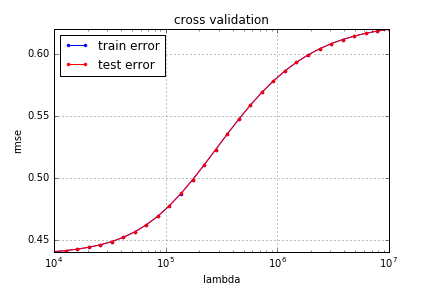
\includegraphics[width=0.47\textwidth]{images/cross_validation.png}
\caption{\small Cross-validation results for test vs training data.}
\label{fig:cross-validation}
\end{figure}

\section{Discussion and Summary}
\label{sec-results}
We applied machine learning techniques to data collected from the CERN particle accelerator aiming at recreating the process of discovering the Higgs particle. We detailed the challenges with the collected data --- many missing values and high dimensionality --- and presented an exploration of pre-filtering and transformation methods for reducing complexity (least significant dimensions) and sample size (outliers), and auto-completion of missing information (mean imputation). We presented the rationale behind an accurate classification based on a combination of algorithms. Our final algorithm can be executed by running \texttt{run.py}. It uses logistic regression with stochastic gradient descent. We cleaned and standardized the data and enriched it by creating a polynomial function of degree 4. This algorithm gave us the following score on Kaggle: $0.81192$ .

%references
\bibliographystyle{unsrt}
\bibliography{report}

\end{sloppypar}
\end{document}